\documentclass[12pt]{article}
\usepackage{lingmacros}
\usepackage{tree-dvips}
\usepackage{url}

\usepackage{pgfplotstable}
\usepackage{pgfplots}
\pgfplotsset{compat = 1.3}
\usepackage{subfig}

\usepackage{amssymb}
\setcounter{tocdepth}{3}
\usepackage{graphicx}

\usepackage{times}
\usepackage{graphicx}
\usepackage{latexsym}
\usepackage{algorithm}
\usepackage{float}
\usepackage[noend]{algpseudocode}
\usepackage{amssymb}
\usepackage{amsmath,amsthm} 
\usepackage{amsfonts}
%%%%%%%\usepackage{mathtools}
\usepackage{verbatim} 
\usepackage{longtable}
\usepackage{graphicx}
\usepackage{booktabs}
\usepackage{epstopdf}
\usepackage{longtable}
\usepackage{pgfpages}
\usepackage{multirow}
\usepackage{varwidth}
%\usepackage{tabularx} % for aligning & numbering equations on the same line
%\usepackage{enumitem}
\usepackage{pifont}


\newcommand{\home}{\texttt{/oledhome}}

\title{OLED Manual}
%\date{}

\begin{document}

\maketitle

\section{Install}
The whole process is illustrated in Figure \ref{fig:terminal}. In detail, do the following:
\begin{itemize}
\item Clone of download the source code from \url{https://github.com/nkatzz/OLED} 
\item Open a terminal and navigate to the location where the source code is cloned. In what follows we'll refer to this directory by \home.
\item From inside \home \ type in the terminal: \\ \texttt{cp -r OLED/install-scripts .}
\item cd into the install-scripts folder and type:\\
\texttt{./install.sh}\\
You will need sudo priviledges to run the install script. The whole process will take some time to complete.
\item If all goes well your \home \ should now look as in Figure \ref{fig:install}. You will use \textsf{oled.jar} to run OLED (see next section).
\item Finally, you'll need to add the path to the \footnotesize \textsf{lpsolve} \normalsize library to your \linebreak \footnotesize \textsf{LD\_LIBRARY\_PATH} \normalsize  variable, the path to the \footnotesize \textsf{LoMRF} \normalsize executable to your \footnotesize \textsf{PATH} \normalsize library and the path to the \footnotesize \textsf{Clingo} \normalsize  executable to your \textsf{PATH} and \footnotesize \textsf{PYTHONPATH} \normalsize variables. To do so, add the lines presented in Figure at the end of your \texttt{/Home/.bashrc} (or your \texttt{/Home/.profile}) file. Don't forget to log-off/log-on again for the updates to the variables to take effect.

\end{itemize}




\begin{figure}[t]
\centering
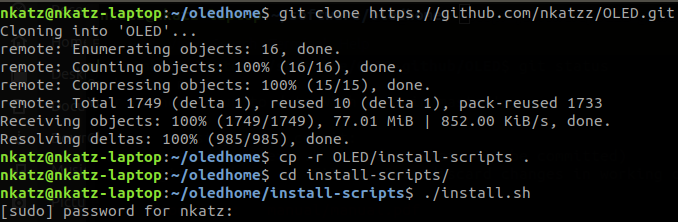
\includegraphics[width=0.8\textwidth]{./figures/install}
\caption{Illustration of the installation process.}%
\label{fig:terminal}
\end{figure}

 

\begin{figure}[t]
\centering
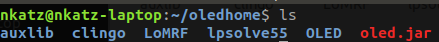
\includegraphics[width=0.6\textwidth]{./figures/install-1}
\caption{Post-installation structure of \home.}%
\label{fig:install}
\end{figure}


\begin{figure}[t]
\centering
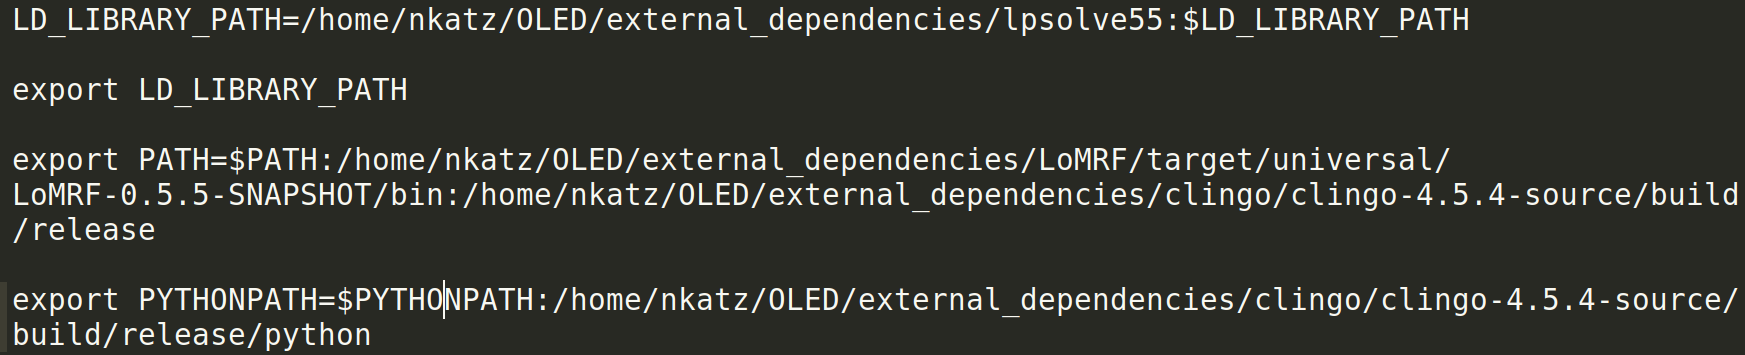
\includegraphics[width=1\textwidth]{./figures/paths}
\caption{Set paths properly at \texttt{/Home/.bashrc} or \texttt{/Home/.profile}.}%
\label{fig:install}
\end{figure}

\section{Run}
We'll next do a test run to make sure that everything is ok. We'll use the CAVIAR\footnote{http://homepages.inf.ed.ac.uk/rbf/CAVIARDATA1/} dataset for human activity recognition. The CAVIAR dataset consists of a number of videos of actors performing a set of activities. Manual annotation (performed by the CAVIAR team) provides ground truth for two activity types. The first type corresponds to simple events and consists of the activities of a person at a certain video frame/time point, such as \emph{walking}, or \emph{standing still}. The second activity type corresponds to complex events and consists of activities that involve more than one person, e.g. two people \emph{meeting each other}, or \emph{moving together}. The goal is to recognize complex events as combinations of simple events and additional contextual knowledge, such as a person's direction and position. 

\subsection{Download and Prepare the Data.}

First, install MongoDB to your computer. We'll use mongo to store the data and consume it in a simulation of a streaming setting. Mongo is very easy to install, just google for specific instructions for your particular Linux distribution.  

\begin{figure}[h]
\centering
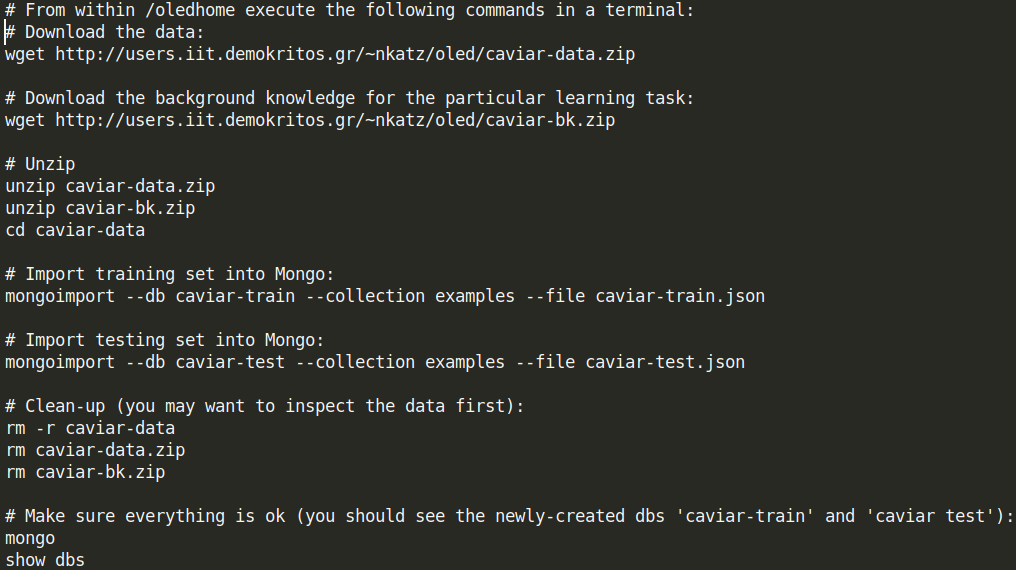
\includegraphics[width=1\textwidth]{./figures/download-caviar}
\caption{Download CAVIAR data and import it into Mongo.}%
\label{fig:caviar}
\end{figure}

Next, download the the data and import it into Mongo. Open a terminal and execute the commands shown in Figure \ref{fig:caviar}. You'll download two datasets, a fragment of CAVIAR that will be used for training (\texttt{caviar-train}) and another that will be used for testing (\texttt{caviar-test}). Subsequently, you'll import each dataset into mongo, clean-up (remove the downloaded data) and make sure that the new dbs were created as required. 

Before cleaning up, you may wish to open the downloaded json files and inspect the data. You'll see that each entry contains three fileds: \texttt{'annotation'}, \texttt{'narrative'} and \texttt{'time'}. The \texttt{'annotation'} filed contains instances of the target complex events we wish to learn definitions for. In this example, we're learning a definition for two persons \emph{meeting each other}, therfore, \texttt{'annotation'} consists of instances of the \emph{meeting} complex event.\linebreak The \texttt{'narrative'} field consists of instances of simple events (\emph{walking}, \emph{active}, \emph{inactive} and so on) and spatiotemporal knowledge, such as persons' coordinates and direction. Each entry is a ``batch'' of data, i.e. it consists of annotation and narrative found within a temporal interval/window. The entry's \texttt{'time'} field is the first time point observed in the batch and it serves as a key to refer to that particular batch/entry.     

Next, take a look at the background knowledge that you downloaded \linebreak (in \texttt{/caviar-bk}). It consists of three files, \texttt{ec}, \texttt{bk} and \texttt{modes}. \texttt{ec} contains the axioms of the Event Calculus. This file is optional in the general case, it is only necessary if you want to learn using the Event Calculus in the backgound knowledge (but it is necessary for the particular test OLED run that we are about to execute). \texttt{bk} is the file where the user defines some domain-specific knowledge. For the purposes of this example, \texttt{bk} contains code for calculating Euclidean distances between persons from their coordinates. Such distances are produced at learning time. All content of the \texttt{ec} and the \texttt{bk} is Answer Set Programming (ASP) code that \texttt{Clingo}, OLED's main reasoning component, is able to execute. Please consult the guide provided by the \texttt{Clingo} team\footnote{Available from \url{https://potassco.org/}, at the documentation site}. The user may use any ASP code in the \texttt{bk} file to define tasks that will be executed by \texttt{Clingo} at learning time, e.g. generating extra, non-input knowledge for the input data, or performing numerical computations via embedded Lua or Python scripts. 

The \texttt{modes} file contains some language bias, i.e. restrictions to the syntax of predicates that may be used to form rules. OLED uses \emph{mode declarations} as a language bias (see the paper that comes with the source code, or any ILP-introductory textbook for details). in addition to the lanhuage bias, the \texttt{modes} file contains a declaration of annotation predicate signatures (via the \texttt{examplePattern/1} predicate) and input predicate signatures (via \texttt{inputPredicate/1}). The latter is the signature specification of all predicates used to pass data to the input and it is used to extract entity types during the learning process. The modes file is necessary for all learning tasks.

We are now ready to perform learning with OLED. cd to your \home \ folder and run the following in a terminal:

\noindent \texttt{java -cp oled.jar app.runners.OLEDDefaultRunner \textbackslash}\\
\texttt{--inpath=/oledhome/caviar-bk --delta=0.00001 \textbackslash}   \\
\texttt{--prune=0.8 --target=meeting --db=caviar-train \textbackslash}\\
\texttt{--saveto=/oledhome/theory.lp}

To see all available command line arguments do \texttt{java -cp oled.jar -help}. The learnt hypothesis will be saved in \texttt{/oledhome/theory.lp}. You may evaluate this theory on the test set as follows: 

\noindent \texttt{java -cp oled.jar app.runners.OLEDDefaultRunner \textbackslash}\\
\texttt{--inpath=/oledhome/caviar-bk --target=meeting \textbackslash}   \\
\texttt{--db=caviar-test --evalth=/oledhome/theory.lp}



\end{document}
